% vim: set tw=78 sts=2 sw=2 ts=8 aw et ai:
Since our previous work has been centered around OLIA and given the poor
performance exposed by a single TCP tunnel, it is only natural that we use the
new testbed in order to gain some insight into this anomaly. Figure
\ref{fig:olia-tcp} summarizes our findings.

\begin{figure}[H]
  \centering
  \subfigure[]{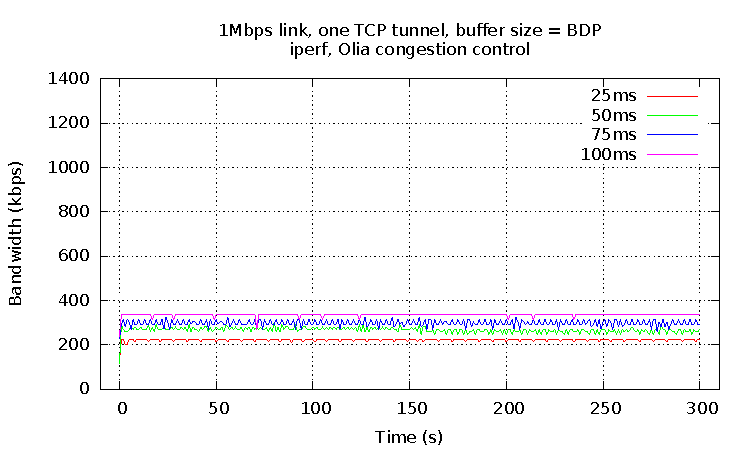
\includegraphics[width=0.45\textwidth]{img/olia-tcp-1}}
  \subfigure[]{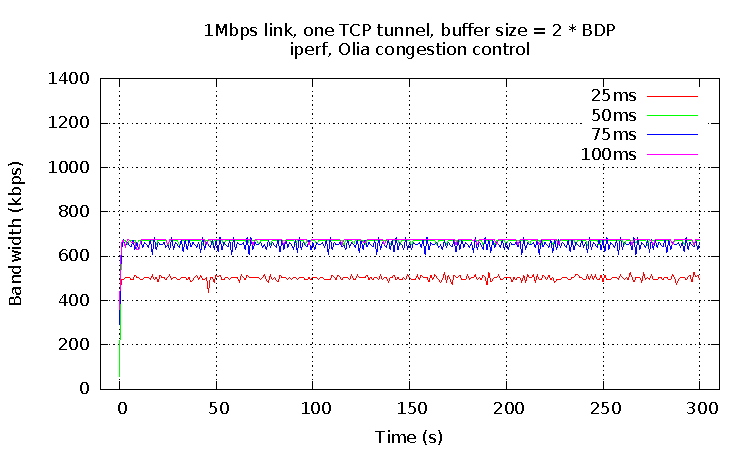
\includegraphics[width=0.45\textwidth]{img/olia-tcp-2}}

  \subfigure[]{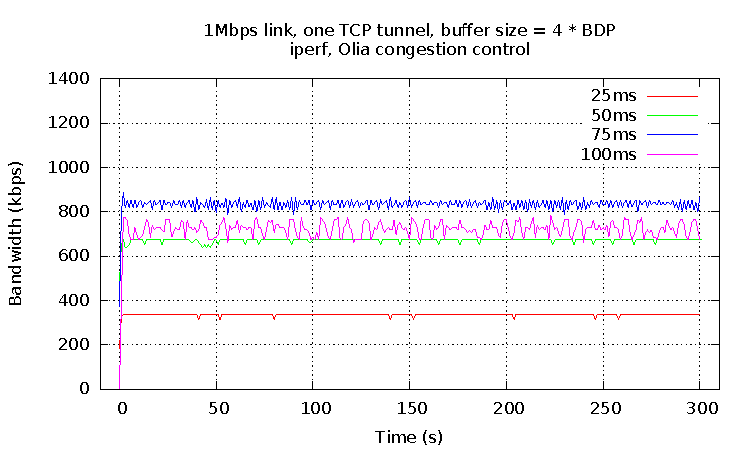
\includegraphics[width=0.45\textwidth]{img/olia-tcp-4}}
  \subfigure[]{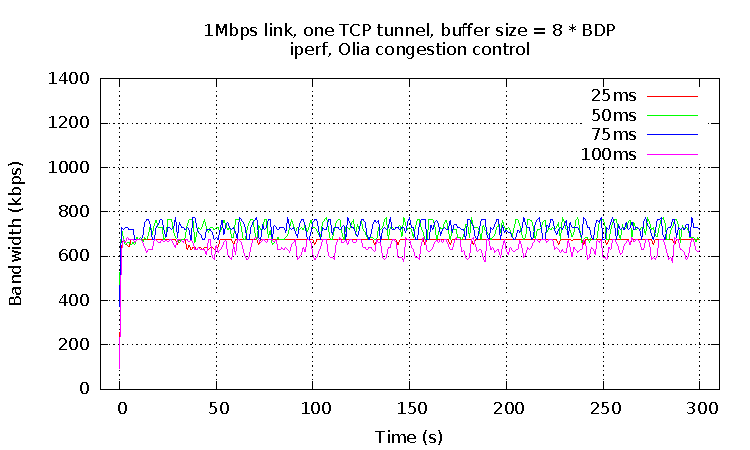
\includegraphics[width=0.45\textwidth]{img/olia-tcp-8}}
  \caption{Single TCP tunnel, OLIA congestion control}
  \label{fig:olia-tcp}
\end{figure}

It is immediately noticeable that the achieved throughput is reasonable. Our
tests show values between 200kbps and 850kbps, given a 1Mbps link and various
delays and buffer sizes. Therefore, the extremely unsatisfactory results
previously noticed can be attributed to the supplementary layer of
virtualization represented by the Mininet framework. It is worth pointing out
that we cannot achieve full link capacity because there is still some
interference between the OpenVPN TCP and the iperf TCP. Additionally, the best
throughput for a single TCP tunnel is gained with a buffer size quadruple of
the BDP. We have taken this into acount when performing the following tests.

Since TCP tunnels running in the new environment are usable we have looked at
the scenario in which a TCP tunnel is used side by side with a UDP tunnel,
both employing buffers equal to the BDP. The results are visible in Figure
\ref{fig:olia-mptcp-1}.

\begin{figure}[H]
  \centering
  \subfigure[25ms delay]{\label{fig:olia-mptcp-1-25}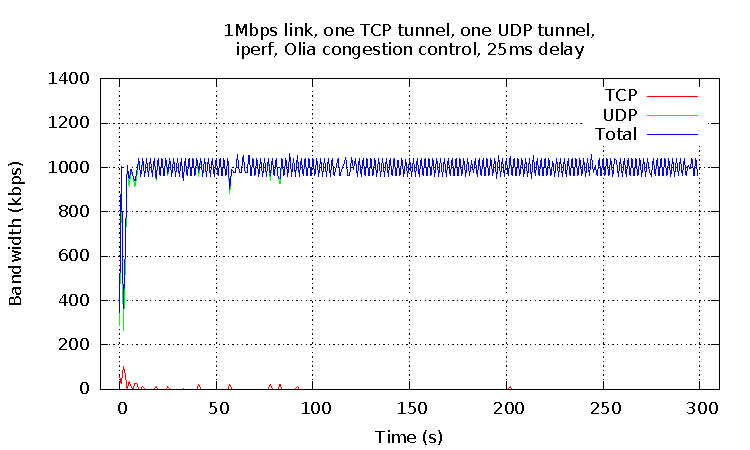
\includegraphics[width=0.45\textwidth]{img/olia-mptcp-25ms}}
  \subfigure[50ms delay]{\label{fig:olia-mptcp-1-50}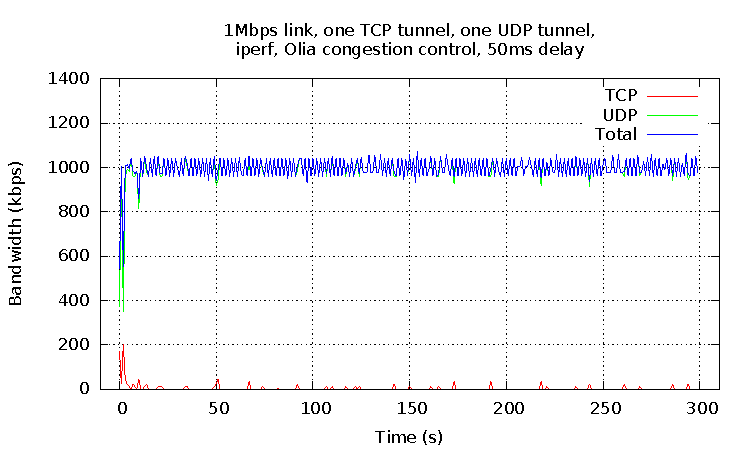
\includegraphics[width=0.45\textwidth]{img/olia-mptcp-50ms}}

  \subfigure[75ms delay]{\label{fig:olia-mptcp-1-75}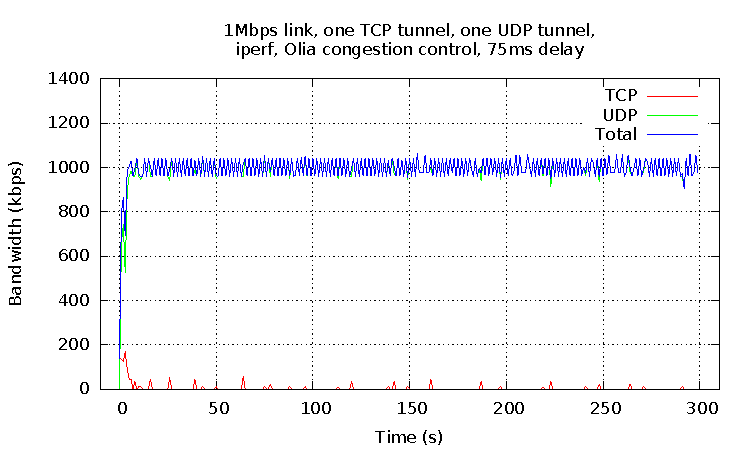
\includegraphics[width=0.45\textwidth]{img/olia-mptcp-75ms}}
  \subfigure[100ms delay]{\label{fig:olia-mptcp-1-100}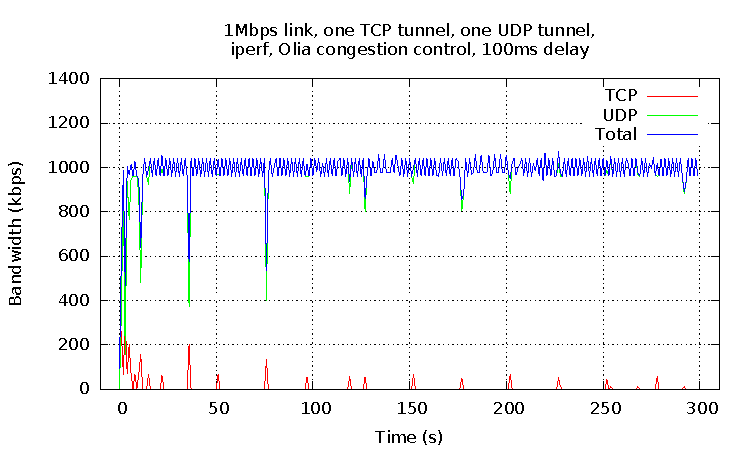
\includegraphics[width=0.45\textwidth]{img/olia-mptcp-100ms}}
  \caption{One TCP tunnel, one UDP tunnel, OLIA congestion control, BDP
  buffer size}
  \label{fig:olia-mptcp-1}
\end{figure}

While is would be expected to see a partition of traffic consistent with the
previous values of roughly 200kbps for the TCP traffic, we notice instead that
traffic is quickly offloaded to the UDP tunnel. This is to be expected, given
the fact that OLIA still identifies the UDP tunnel as being more suitable for
sending data. In fact, this behavior is noticeable even if we change the TCP
tunnel buffer size to quadruple the BDP, as seen in Figure
\ref{fig:olia-mptcp-4}. While initially more traffic is sent via the TCP
tunnel, in agreement with our single TCP tunnel tests, data is just as quickly
shifted to the UDP tunnel.

The previous benchmarks have been synthetic and their goal was to precisely
highlight how specific factors influence MPTCP tunnels. However, we have
looked at a real world scenario, namely a mobile device with WiFi and 3G
connectivity. Previous research\cite{latencies} has shown that WiFi links can
have 50ms delays and 3G links can go up to 200ms delay times. We have
simulated these conditions, while taking into account the findings from
previous tests. That is, we ran a test with a TCP tunnel and a UDP tunnel,
each having its own buffer size and delay. The result can be seen in Figure 5.

\begin{figure}[H]
  \centering
  \subfigure[25ms delay]{\label{fig:olia-mptcp-4-25}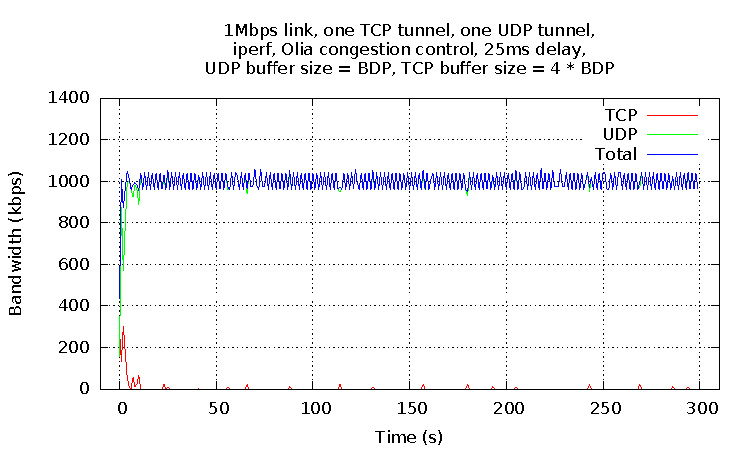
\includegraphics[width=0.45\textwidth]{img/olia-mptcp-25ms-4}}
  \subfigure[50ms delay]{\label{fig:olia-mptcp-4-50}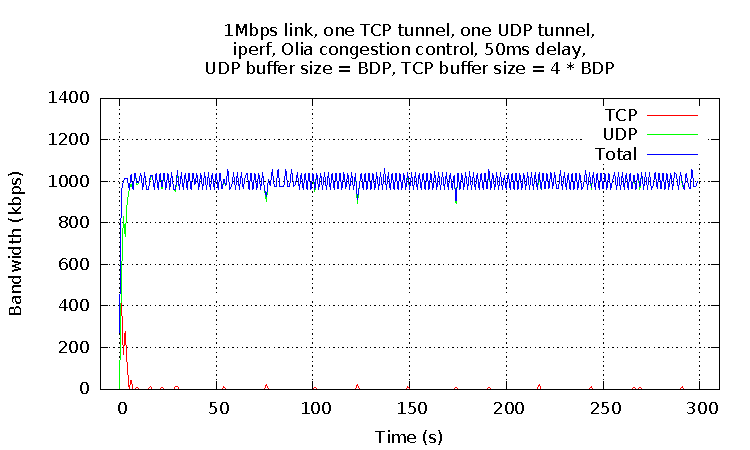
\includegraphics[width=0.45\textwidth]{img/olia-mptcp-50ms-4}}

  \subfigure[75ms delay]{\label{fig:olia-mptcp-4-75}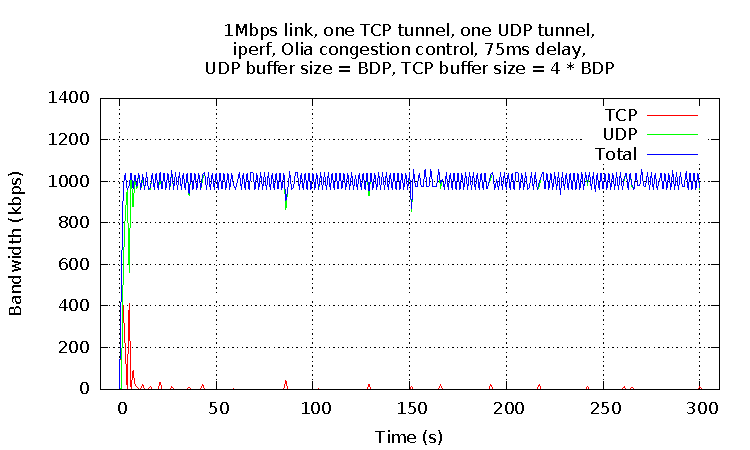
\includegraphics[width=0.45\textwidth]{img/olia-mptcp-75ms-4}}
  \subfigure[100ms delay]{\label{fig:olia-mptcp-4-100}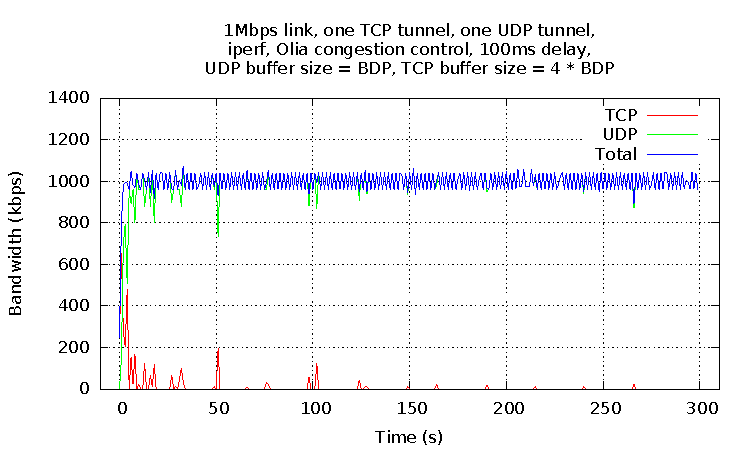
\includegraphics[width=0.45\textwidth]{img/olia-mptcp-100ms-4}}
  \caption{One TCP tunnel, one UDP tunnel, OLIA congestion control, 4xBDP
  buffer size}
  \label{fig:olia-mptcp-4}
\end{figure}

\begin{figure}[H]
  \centering
  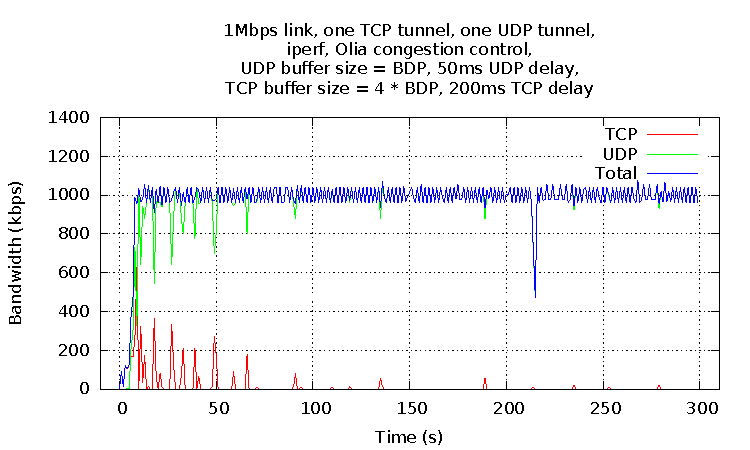
\includegraphics[width=0.8\textwidth]{img/olia-mptcp-unequal}
  \label{fig:mobile-olia}
  \caption{Simulated WiFi/3G test, OLIA congestion control}
\end{figure}

We have ran the same battery of tests for the wVegas since it employs a
different strategy for detecting collisions. Figure \ref{fig:wvegas-tcp} shows
the behavior of a single TCP tunnel. 

\begin{figure}[H]
  \centering
  \subfigure[]{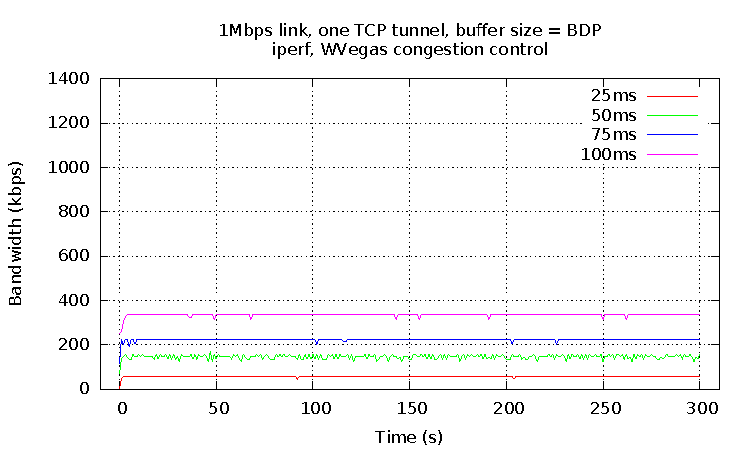
\includegraphics[width=0.45\textwidth]{img/wvegas-tcp-1}}
  \subfigure[]{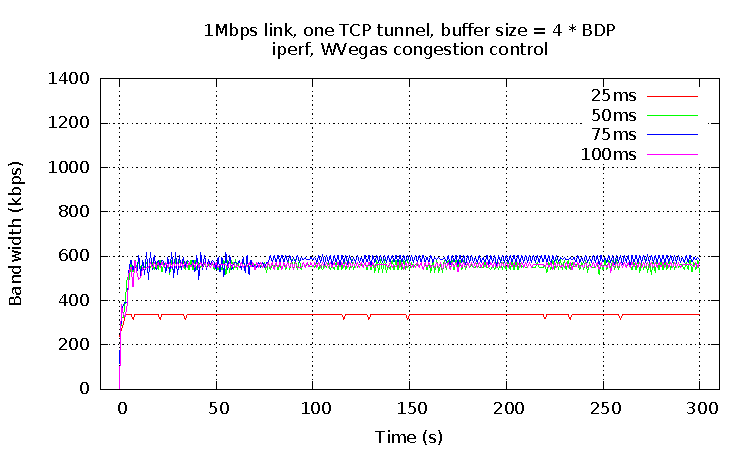
\includegraphics[width=0.45\textwidth]{img/wvegas-tcp-4}}
  \caption{Single TCP tunnel, wVegas congestion control}
  \label{fig:wvegas-tcp}
\end{figure}

We have only tested for regular and quadruple buffer sizes since they have
yielded the minimum and maximum throughput when testing with OLIA. Comparing
the two algorithms, it is obvious that OLIA performs better in terms of
throughput. However, it is worth noticing that wVegas throughput, albeit
smaller, is more stable across the 5 minute test time. We attribute this to
the fact that wVegas looks at delay instead of packet losses to detect
congestion and therefore is not so easily affected by the interference
generated by running TCP over TCP.

This characteristic of wVegas manifests itself more proeminently in our tests
with both TCP and UDP tunnels, especially in the case of the TCP tunnel having
a buffer size four times the BDP. Figures \ref{fig:wvegas-mptcp-1}
and \ref{fig:wvegas-mptcp-4} outline its contribution to the overall
throughput.

\begin{figure}[H]
  \centering
  \subfigure[25ms delay]{\label{fig:wvegas-mptcp-1-25}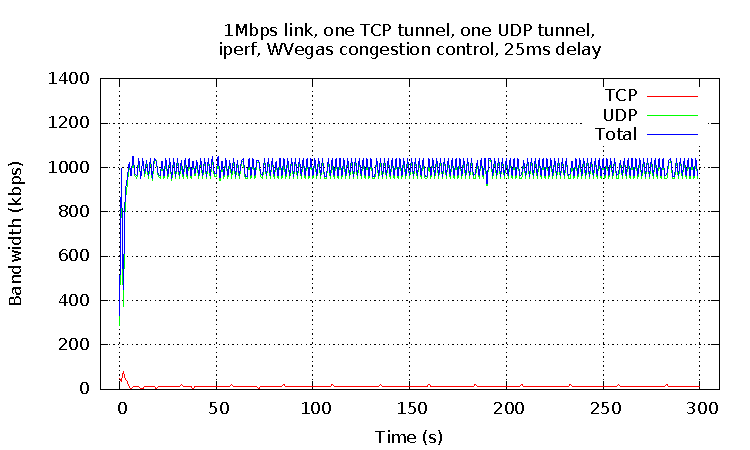
\includegraphics[width=0.45\textwidth]{img/wvegas-mptcp-25ms}}
  \subfigure[50ms delay]{\label{fig:wvegas-mptcp-1-50}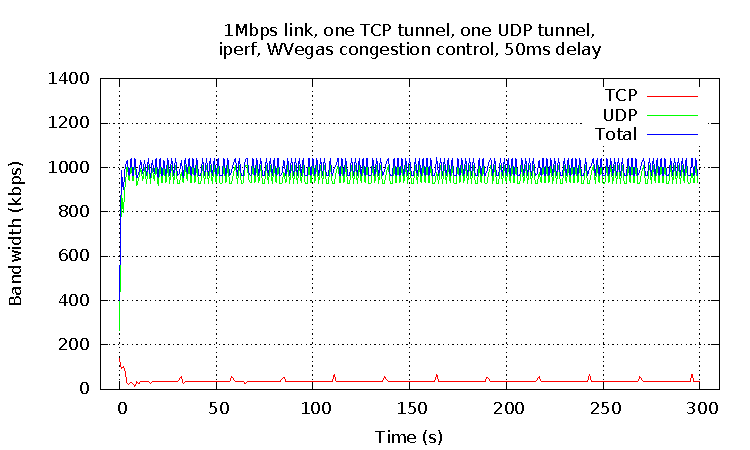
\includegraphics[width=0.45\textwidth]{img/wvegas-mptcp-50ms}}

  \subfigure[75ms delay]{\label{fig:wvegas-mptcp-1-75}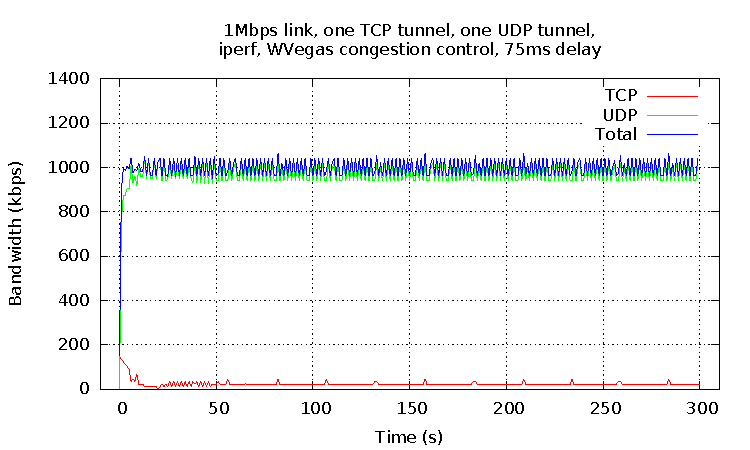
\includegraphics[width=0.45\textwidth]{img/wvegas-mptcp-75ms}}
  \subfigure[100ms delay]{\label{fig:wvegas-mptcp-1-100}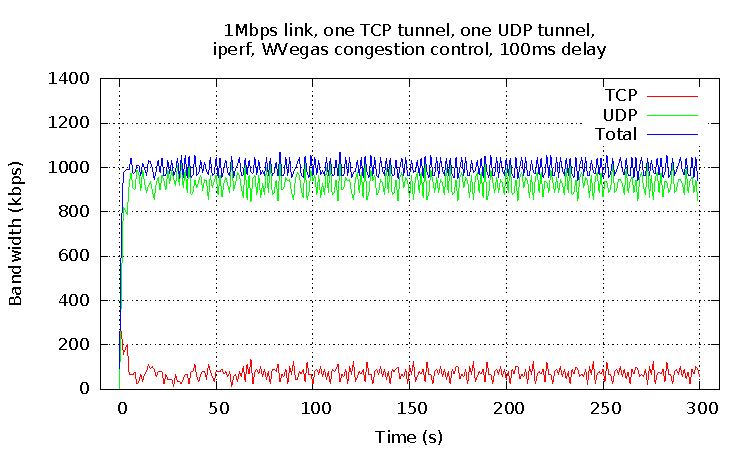
\includegraphics[width=0.45\textwidth]{img/wvegas-mptcp-100ms}}
  \caption{One TCP tunnel, one UDP tunnel, wVegas congestion control, BDP
  buffer size}
  \label{fig:wvegas-mptcp-1}
\end{figure}

\begin{figure}[H]
  \centering
  \subfigure[25ms delay]{\label{fig:wvegas-mptcp-4-25}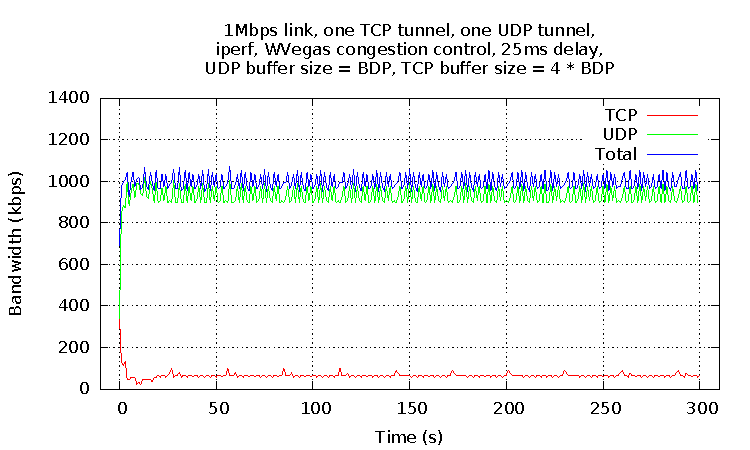
\includegraphics[width=0.45\textwidth]{img/wvegas-mptcp-25ms-4}}
  \subfigure[50ms delay]{\label{fig:wvegas-mptcp-4-50}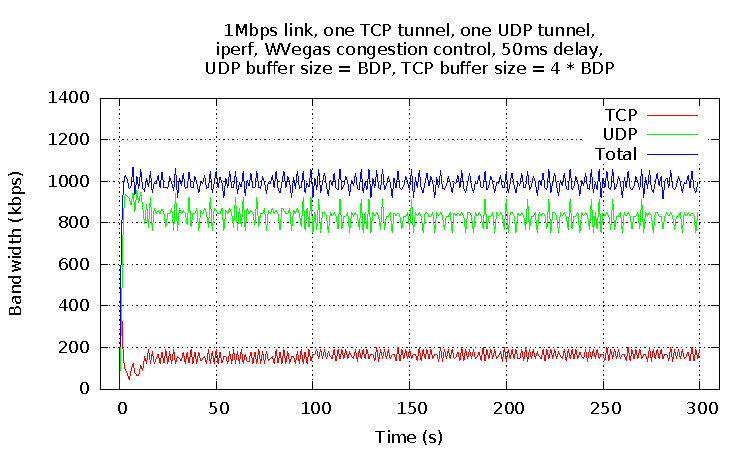
\includegraphics[width=0.45\textwidth]{img/wvegas-mptcp-50ms-4}}

  \subfigure[75ms delay]{\label{fig:wvegas-mptcp-4-75}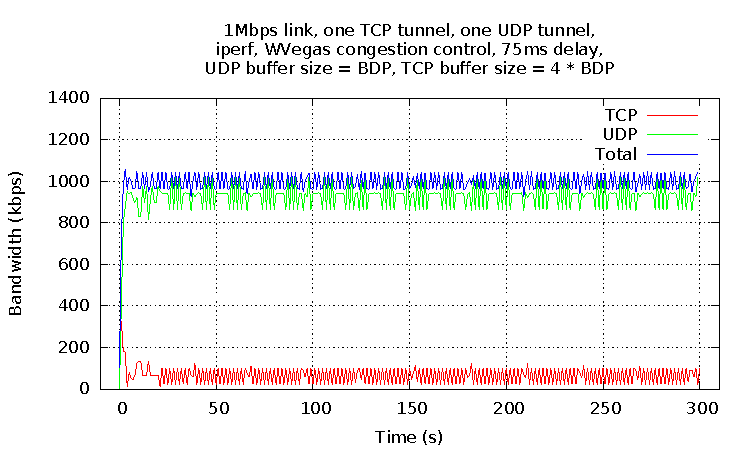
\includegraphics[width=0.45\textwidth]{img/wvegas-mptcp-75ms-4}}
  \subfigure[100ms delay]{\label{fig:wvegas-mptcp-4-100}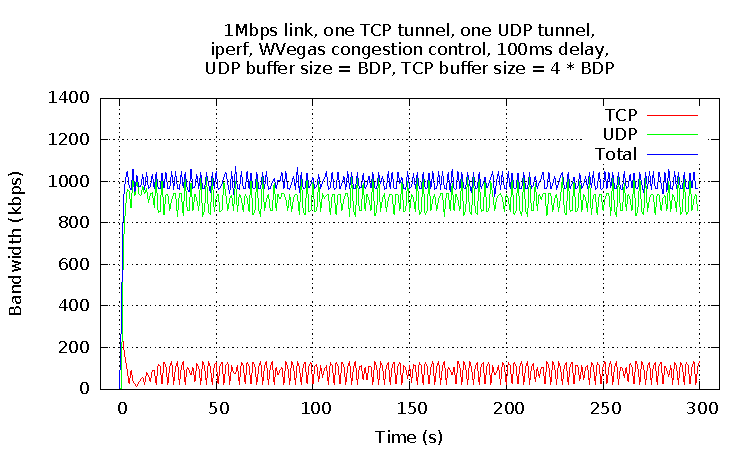
\includegraphics[width=0.45\textwidth]{img/wvegas-mptcp-100ms-4}}
  \caption{One TCP tunnel, one UDP tunnel, wVegas congestion control, 4xBDP
  buffer size}
  \label{fig:wvegas-mptcp-4}
\end{figure}

While using OLIA, traffic is shifted early on in the test over to the UDP
tunnel. However, when using wVegas, up to 200kbps of the throughput is handled
by the TCP tunnel during the full 5 minutes test time. This is again a
consequence of the wVegas congestion control strategy.

We have also considered the WiFi/3G scenario for wVegas, as can be observed in
Figure 9.

\begin{figure}[H]
  \centering
  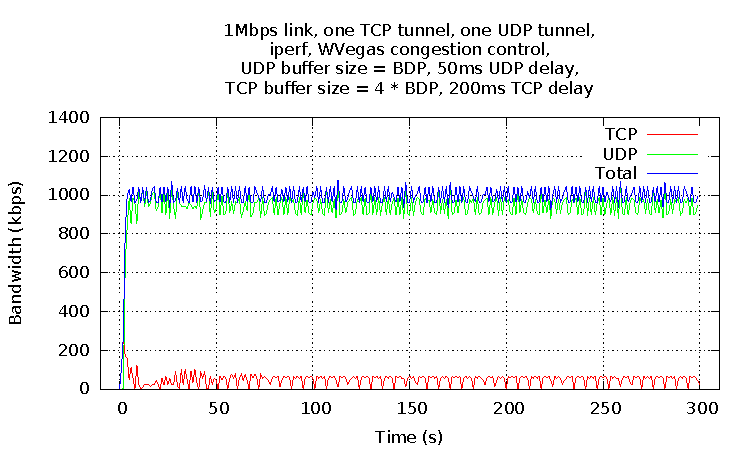
\includegraphics[width=0.8\textwidth]{img/wvegas-mptcp-unequal}
  \label{fig:mobile-wvegas}
  \caption{Simulated WiFi/3G test, wVegas congestion control}
\end{figure}

The same stability of throughput compared to OLIA can be noticed in the
WiFi/3G test. However, the TCP delay is 4 times greater than the UDP delay.
This is enough to make wVegas shift traffic over to the UDP tunnel, so we do
not achieve a traffic partition on par with the synthetic tests.
